% 
% exemplo genérico de uso da classe iiufrgs.cls
% $Id: iiufrgs.tex,v 1.1.1.1 2005/01/18 23:54:42 avila Exp $
% 
% This is an example file and is hereby explicitly put in the
% public domain.
% 
\documentclass[tuberlin,cic,tc,openright,english,noabntcite,oneside]{iiufrgs}
% Para usar o modelo, deve-se informar o programa e o tipo de documento.
% Programas :
% * cic       -- Graduação em Ciência da Computação
% * ecp       -- Graduação em Ciência da Computação
% * ppgc      -- Programa de Pós Graduação em Computação
% * pgmigro   -- Programa de Pós Graduação em Microeletrônica
% * tuberlin  -- Bachelorarbeit entregue na TU Berlin
% 
% Tipos de Documento:
% * tc                -- Trabalhos de Conclusão (apenas cic e ecp)
% * diss ou mestrado  -- Dissertações de Mestrado (ppgc e pgmicro)
% * tese ou doutorado -- Teses de Doutorado (ppgc e pgmicro)
% * ti                -- Trabalho Individual (ppgc e pgmicro)
% 
% Outras Opções:
% * english    -- para textos em inglês
% * openright  -- Força início de capítulos em páginas ímpares (padrão da
% biblioteca)
% * oneside    -- Desliga frente-e-verso
% * nominatalocal -- Lê os dados da nominata do arquivo nominatalocal.def


% Use unicode
\usepackage[utf8]{inputenc}   % pacote para acentuação
\usepackage[german,english]{babel}

% Necessário para incluir figuras
\usepackage{graphicx}         % pacote para importar figuras
\usepackage{float}
\usepackage{subcaption}
\graphicspath{ {img/} }
\setlength{\intextsep}{1\baselineskip} % evita espaços antes e depois de floats
\setlength{\belowcaptionskip}{10pt plus 3pt minus 2pt} % espaço depois de caption

\usepackage{times}            % pacote para usar fonte Adobe Times
% \usepackage{palatino}
% \usepackage{mathptmx}       % p/ usar fonte Adobe Times nas fórmulas

%\usepackage[alf,abnt-emphasize=bf]{abntex2cite}	% pacote para usar citações abnt
\usepackage[autostyle,english=american]{csquotes}
\usepackage[authordate,backend=biber,refsection=chapter]{biblatex-chicago}
\addbibresource{biblio.bib}

% Para algoritmos
\usepackage{amsfonts}
\usepackage{algpseudocode}
\usepackage{algorithm}
\usepackage{algorithmicx}

% Matemáticas
\usepackage{amsmath}
\usepackage{amsthm}
\newtheorem{definition}{Definition}
\allowdisplaybreaks

% Linear Programming
%----------------------------------------------------------------------------------------
%	Macros para definir programa linear
%----------------------------------------------------------------------------------------
\makeatletter
\newcommand{\minproblem}{\@ifstar\minproblemstar\minproblemplain}
\newcommand{\minproblemplain}[3][]{
  \begin{align}
    \text{#1}\textbf{minimize}\qquad & #2\\
    \textbf{subject to}\qquad & #3
  \end{align}
}
\newcommand{\minproblemstar}[3][]{
  \begin{align*}
    \text{#1}\textbf{minimize}\qquad & #2\\
    \textbf{subject to}\qquad & #3
  \end{align*}
}
\newcommand{\maxproblem}{\@ifstar\maxproblemstar\maxproblemplain}
\newcommand{\maxproblemplain}[3][]{
  \begin{align}
    \text{#1}\textbf{maximize}\qquad & #2\\
    \textbf{subject to}\qquad & #3
  \end{align}
}
\newcommand{\maxproblemstar}[3][]{
  \begin{align*}
    \text{#1}\textbf{maximize}\qquad & #2\\
    \textbf{subject to}\qquad & #3
  \end{align*}
}
\makeatother
\renewcommand\theequation{\arabic{equation}}

% 
% Informações gerais
% 
\title{Solving the Dial-a-Ride Problem with the Firefly Metaheuristic}

\author{Bombardelli da Silva}{Fernando}
% alguns documentos podem ter varios autores:
% \author{Flaumann}{Frida Gutenberg}
% \author{Flaumann}{Klaus Gutenberg}

% orientador e co-orientador são opcionais (não diga isso pra eles :))
\advisor[Dr.-Ing.]{Heßler}{Axel}
\reviewer[Prof. Dr. Dr. h.c.]{Albayrak}{Sahin}
\reviewer[Prof. Dr. habil.]{Kao}{Odej}

% a data deve ser a da defesa; se nao especificada, são gerados
% mes e ano correntes
% \date{maio}{2001}

% o local de realização do trabalho pode ser especificado (ex. para TCs)
% com o comando \location:
\location{Berlin}{Germany}

% itens individuais da nominata podem ser redefinidos com os comandos
% abaixo:
% \renewcommand{\nominataReit}{Prof\textsuperscript{a}.~Wrana Maria Panizzi}
% \renewcommand{\nominataReitname}{Reitora}
% \renewcommand{\nominataPRE}{Prof.~Jos{\'e} Carlos Ferraz Hennemann}
% \renewcommand{\nominataPREname}{Pr{\'o}-Reitor de Ensino}
% \renewcommand{\nominataPRAPG}{Prof\textsuperscript{a}.~Joc{\'e}lia Grazia}
% \renewcommand{\nominataPRAPGname}{Pr{\'o}-Reitora Adjunta de P{\'o}s-Gradua{\c{c}}{\~a}o}
% \renewcommand{\nominataDir}{Prof.~Philippe Olivier Alexandre Navaux}
% \renewcommand{\nominataDirname}{Diretor do Instituto de Inform{\'a}tica}
% \renewcommand{\nominataCoord}{Prof.~Carlos Alberto Heuser}
% \renewcommand{\nominataCoordname}{Coordenador do PPGC}
% \renewcommand{\nominataBibchefe}{Beatriz Regina Bastos Haro}
% \renewcommand{\nominataBibchefename}{Bibliotec{\'a}ria-chefe do Instituto de Inform{\'a}tica}
% \renewcommand{\nominataChefeINA}{Prof.~Jos{\'e} Valdeni de Lima}
% \renewcommand{\nominataChefeINAname}{Chefe do \deptINA}
% \renewcommand{\nominataChefeINT}{Prof.~Leila Ribeiro}
% \renewcommand{\nominataChefeINTname}{Chefe do \deptINT}

% A seguir são apresentados comandos específicos para alguns
% tipos de documentos.

% Relatório de Pesquisa [rp]:
% \rp{123}             % numero do rp
% \financ{CNPq, CAPES} % orgaos financiadores

% Trabalho Individual [ti]:
% \ti{123}     % numero do TI
% \ti[II]{456} % no caso de ser o segundo TI

% Monografias de Especialização [espec]:
% \espec{Redes e Sistemas Distribuídos}      % nome do curso
% \coord[Profa.~Dra.]{Weber}{Taisy da Silva} % coordenador do curso
% \dept{INA}                                 % departamento relacionado

% 
% palavras-chave
% iniciar todas com letras minúsculas, exceto no caso de abreviaturas
% 
\keyword{Dial-a-ride problem}
\keyword{Firefly algorithm}
\keyword{Metaheuristic}
\keyword{Integer programming}
\keyword{Vehicle routing}

%\settowidth{\seclen}{1.10~}

% 
% inicio do documento
% 
\begin{document}

% folha de rosto
% às vezes é necessário redefinir algum comando logo antes de produzir
% a folha de rosto:
% \renewcommand{\coordname}{Coordenadora do Curso}
\maketitle

% dedicatoria
% \clearpage
% \begin{flushright}
%     \mbox{}\vfill
%     {\sffamily\itshape
%       ``If I have seen farther than others,\\
%       it is because I stood on the shoulders of giants.''\\}
%     --- \textsc{Sir~Isaac Newton}
% \end{flushright}

% agradecimentos
%\chapter*{Agradecimentos}
%Agradeço ao \LaTeX\ por não ter vírus de macro\ldots



% resumo na língua do documento
\begin{abstract}
The Dial-a-ride problem (DARP) is an $\mathcal{NP}$-hard combinatorial optimization problem with practical applications in user-oriented public transportation. The DARP is a vehicle routing problem whose instances consist of a set of vehicles and a set of pick-up and drop-off requests from passengers. Its goal is to assign the requests to the vehicles and to calculate the routes of each one of them, minimizing the operation costs and ensuring that all the constraints, such as vehicle capacity, departure and arrival time windows, and maximal user ride time, are fulfilled. This work presents a mathematical formulation of the problem and seeks to solve it through the firefly algorithm (FA). The FA is a novel nature-based metaheuristic inspired by the behavior of fireflies, which applies the concept of swarm intelligence in order to optimize mathematical functions by looking for near-optimal solutions. With the aid of this technique we aimed to model and implement a solver to the DARP which explores the huge combinatorial search space, generated by the problem instances, in an efficient way. Finally, we carried out a performance comparison between the proposed method and the algorithms found in the scientific literature, what pointed out that the former achieves an average of 90\% of optimality for a specific set of instances, and delivers, in some experiments, faster results than those delivered by one of the algorithms from the literature.
\end{abstract}

% resumo na outra língua
% como parametros devem ser passados o titulo e as palavras-chave
% na outra língua, separadas por vírgulas
\begin{englishabstract}{Lösung des Dial-a-Ride-Problems mit der Firefly-Metaheuristik}{Dial-a-Ride-Problem. Firefly-Algorithmus. Metaheuristik. Ganzzahlige Optimierung. Tourenplanung}
Das Dial-a-Ride-Problem ist ein $\mathcal{NP}$-schweres kombinatorisches Optimierungsproblem, das bei benutzerorientiertem öffentlichen Personenverkehr Anwendung findet. Das DARP ist ein Tourenplanungsproblem, dessen Instanzen aus einer Menge von Fahrzeugen und einer Menge von von Fahrgästen eingetragenen Aufträgen zum Abholen und zum Absetzen bestehen. Sein Ziel ist es, den Fahrzeugen die Aufträge zuzuweisen und die Routen jedes Wagens zu berechnen, sodass die Betriebskosten minimiert werden und jede Beschränkung, wie z.B. Fahrzeugnutzlast, Zeitfenster für Ein- und Ausstieg, maximale Fahrtdauer, erfüllt werden. Diese Arbeit stellt eine mathematische Formulierung des Problems vor und versucht, es durch den Einsatz des Firefly-Algorithmus (FA) zu lösen. Der FA ist eine neue naturbasierte Metaheuristik, die vom Verhalten von Glühwürmchen inspiriert ist und das Konzept von Schwarmintelligenz anwendet, um mathematische Funktionen zu optimieren, indem sie quasi-optimale Lösungen sucht. Anhand dieses Verfahrens hat diese Arbeit einen Löser des DARP modelliert und implementiert, der den riesigen kombinatorischen, von Problemintanzen generierten Suchraum effizienterweise erforscht. Letztendlich wurde ein Leistungsvergleich zwischen der vorgeschlagenen Methode und den Algorithmen aus der wissenschaftlichen Literatur durchgeführt, der darauf hinwies, dass die vorgeschlagene Methode einen Durchschnitt von 90\% von Optimalität für eine bestimmte Menge von Instanzen erreicht und in einigen Experimenten schnellere Ergebnisse liefert, als die von einem der Algorithmen, die von der Lietratur stammen, gelieferten Ergebnisse.
\end{englishabstract}

% lista de figuras
\listoffigures

% lista de tabelas
\listoftables

% lista de abreviaturas e siglas
% o parametro deve ser a abreviatura mais longa
\begin{listofabbrv}{MD-H-DARP}
	\item[AMPL] A Mathematical Programming Language
	\item[CPU] Central Processing Unit
    \item[DARP] Dial-a-Ride Problem
    \item[FA] Firefly Algorithm
    \item[GA] Genetic Algorithms
    \item[GLPK] GNU Linear Programming Kit
    \item[MD-H-DARP] Multi-Depot Heterogeneous Dial-A-Ride Problem
    \item[PDVRP] Pickup and Delivery Vehicle Routing Problem
    \item[PSO] Particle Swarm Optimization
    \item[RAM] Random Access Memory
    \item[VRPTW] Vehicle Routing Problem with Time Windows
\end{listofabbrv}

% idem para a lista de símbolos
% \begin{listofsymbols}{$\alpha\beta\pi\omega$}
%     \item[$\sum{\frac{a}{b}}$] Somatório do produtório
%     \item[$\alpha\beta\pi\omega$] Fator de inconstância do resultado
% \end{listofsymbols}

% sumario
\tableofcontents

% aqui comeca o texto propriamente dito

%============================================================
% Chapter 1. Introduction
%============================================================
\chapter{Introduction}
In current urban areas, mainly in very populated cities, there is a considerable number of mobility problems. These problems have been seen with much interest by the scientific community, which has been strongly contributing to the improvement of transportation and logistic networks, thus promoting advances towards a better urban mobility.

The problem addressed here is referred to as the \textbf{Dial-a-ride problem (DARP)}. Shortly, it consists of a system with a set of requests for pick-up and delivery, that are entered by passengers, and a fleet of vehicles. The goal is to plan the route of the vehicles and the assignment of requests to them in a feasible way, what means fulfilling the constraints of both the requests and the vehicles, which a feasible solution is subject to. These can be several conditions, such as location and time limit for picking up and delivering, or for how much time each vehicle can operate. Besides, not only a feasible solution is searched but also an optimal one that minimizes the operation costs, defined by the so-called objective function. In this work, as in the literature, the total time of operation represents the objective function to be minimized.

Many difficulties are found when trying to solve the described problem, mainly because it belongs to the so-called $\mathcal{NP}$-hard class of problems, as proven by \textcite{baugh_jr._intractability_1998}. Therefore, the combinatorial nature of its solution space makes the DARP hard to be solved for large inputs due to its high complexity. As a consequence, one might find major difficulty in building a scalable application in order to solve it.

\section{Definition}
\textcite[p. 29]{cordeau_dial--ride_2007} states the problem very briefly in this way:
\begin{quote}
\enquote{The Dial-a-Ride Problem (DARP) consists of designing vehicle routes and schedules for $n$ users who specify pick-up and delivery requests between origins and destinations. The aim is to plan a set of $m$ minimum cost vehicle routes capable of accommodating as many users as possible, under a set of constraints.}
\end{quote}

The author summarizes the subject very well, however, a closer look is to be taken. The instances of the problem specify the following properties, that are taken as input by the solver. Firstly, the system has available an \textbf{amount of homogeneous vehicles}, that is to say, no distinction should be made regarding possible vehicle types. Secondly, there is a \textbf{single depot}, where the vehicles start from and where they end their routes. Next, the cars have the attributes of \textbf{maximal route duration time} and \textbf{capacity}, which tell how many passengers a vehicle can carry at a time. The passengers have a \textbf{maximum allowed travel time}, that serves to guarantee their comfort. Finally, there are $n$ \textbf{requests}, which have the following features:

\begin{itemize}
\item Pick-up location;
\item Drop-off location;
\item Time window for picking up (a time interval in which the vehicle is expected to be at the site);
\item Time window for dropping off;
\item Time needed for boarding or alighting;
\item Quantity of passengers;
\end{itemize}

Additionally, it is possible for a car to move from every location to any other location, and the time needed to travel between any pair is considered to be the linear distance between these two points. In real-world applications data from the geographical region and from traffic could be taken into account, but, by reason of abstraction, this model will not consider this kind of information.

To sum up, the abovementioned parameters form the constraints of the problem, which a solver shall consider. But, regarding the goal, two concepts are still to be elucidated in order to define it, namely feasible and optimal solution. The former is defined thusly:
\begin{definition}[Feasible solution]
Determination of the routes of the vehicles, in such a way that, every request is picked up, transported and then delivered by one and only one vehicle, and all the conditions of the problem are fulfilled.
\end{definition}

In order to make it clearer, let a route be defined as:
\begin{definition}[Route]
The order of the locations through which a vehicle travels. The first and the last location is the depot and a vehicle must be able to execute the whole journey without breaking the conditions of time windows of the requests assigned to it.
\end{definition}

Finally, one can calculate the duration time of the operation for every feasible solution by basically summing up the duration times of every vehicle route. Based on this, the optimal solution is defined as follows.
\begin{definition}[Optimal solution]
A feasible solution whose duration time is less than or equal to any other feasible solution's duration time.
\end{definition}

In conclusion, the goal of the Dial-a-ride problem is to find an optimal solution for a given instance.

\section{Approach}
In this work two approaches shall be taken in order to solve the optimization problem. The exact approach consists in mathematically modeling the DARP as an \textbf{integer linear program} and then transcribing it into a \textbf{mathematical programming language} aiming to execute it with a generic linear programming solver. The near-optimal approach shall then analyze and develop a program that implements the \textbf{firefly metaheuristic} to efficiently seek near-optimal solutions.

Finally, the goal of the research is: (i) to compare the performance of the two different models, both through the execution time and through the solution quality as well as through the possibility of dealing with large inputs; (ii) to conduct an evaluation of the firefly metaheuristic implementation capabilities when solving the instances used in other works of the literature.

\section{Justification}
It is expected that the results of this work might bring relevant contributions to the handling of the presented problem, and even of other ones. By having two distinct approaches, it is possible to compare results regarding important features of the problem, such as scalability, feasibility and deviation to an optimal solution. Furthermore, applying the relatively new firefly algorithm to the problem can show how it performs in a such a discrete and complex solution space.

In addition to the contributions to the understanding of the behavior of swarm metaheuristics applied to optimization problems of transportation, the new procedure of solving the problem serves as a prototype and brings a new perspective to commercial applications which seek constantly to treat the problem in a more efficient and scalable way.

With regard to the current cities' mobility, there is a growing demand for an efficient alternative to the classical means of transportation. The implementation of such a system improves the possibility of mobility of the population and makes it more efficient, since it allows the decrease of the number of cars that drive every day through the urban network causing traffic jams in big cities. Moreover, it helps to solve a demanding problem in today's society where there is an increasing number of elderly or handicapped people, who have the right to mobility and need assistance to travel in the town.

Also in an economical view, this research contributes to the win of new markets by companies that aim to enter the branch of public transportation since its main goal is minimizing the operation costs. With a business model based on the reduction of transaction costs, a company can take great advantages against competitors in order to capture marketplace.

At last, the proposed model shows also an ecological concern since it enables the decrease of greenhouse gases emissions, such as the CO$_{2}$, in urban areas by two reasons: Firstly, by minimizing operation costs, thus, minimizing the burning of fossil fuels, and secondly, by reducing the volume of the circulation of taxis and private automobiles.

%============================================================
% Chapter 2. Literature Review
%============================================================
\chapter{Literature Review}
According to \textcite[p. 30]{cordeau_dial--ride_2007}, the Dial-a-ride Problem (DARP) is very similar to other problems studied by computer scientists, namely the \emph{Pickup and Delivery Vehicle Routing Problem} (PDVRP) and the \emph{Vehicle Routing Problem with Time Windows} (VRPTW), problems that have application in logistics. The authors point out that, what basically differs the DARP from these other problems is the human perspective, by the fact that people are transported. This often appears having two distinct goals, minimizing operation costs, subject to the constraints, and maximizing the availability and quality of the service. The quality criteria include frequently aspects, like route duration, customer waiting and ride time, maximum vehicle ride time, among others, and are usually treated as the constraints of the optimization problem.

\textcite{cordeau_dial--ride_2007} realized a survey on the subject, wherein they showed the distinctions between the several approaches and formulations of the problem. Firstly, the DARP occurs in a \textbf{static} version in which the requests are known beforehand, this is the one that we treat here, alternatively, there is a \textbf{dynamic} version, dealt by \textcite{berbeglia_dynamic_2010}, in which requests can be entered during the operation of the transportation service.

Another distinction to be made is between the \textbf{homogeneous} and the \textbf{heterogeneous} Dial-a-ride Problem. The former proceeds on the assumption that every vehicle is equal. The latter, on the other hand, distinguishes the vehicles either in capacity or in additionally features, such as space for wheelchair  \parencite[p. 593]{parragh_models_2012}. In the same way, the objectives can differ by aiming \textbf{cost minimization} or \textbf{satisfied demand maximization} \parencite[p. 30]{cordeau_dial--ride_2007}. \textcite{urra_hyperheuristic_2015} have succeeded on handling the second one. A last differentiation of the problem is done regarding the depots, which can be a \textbf{single} one or \textbf{multiple} ones, in this case referred to as \emph{Multi-Depot Heterogeneous Dial-A-Ride Problem} (MD-H-DARP) \parencite[p. 166]{braekers_exact_2014}.

In their survey, \textcite{cordeau_dial--ride_2007} identified in the literature three formulations. Two of them are described as a mathematical linear program and the other one as a scheduling problem. The \textbf{three-index mathematical formulation}, proposed by \textcite{cordeau_branch-and-cut_2006}, uses binary three-index variables $x_{i,j}^{k}$ to assign routes to each bus and then to minimize costs. In addition, \textcite{ropke_models_2007} came up with a \textbf{two-index formulation} which reduces the number of variables, thus, allowing the exact solution approach to be more efficient.

Exact algorithms have been proposed by several researchers, to highlight are the \textbf{branch-and-cut} by \textcite{cordeau_branch-and-cut_2006}, and also by \textcite{ropke_models_2007}. Lately \textcite{parragh_hybrid_2013} were successful in solving the DARP with an exact approach that uses \textbf{large neighborhood search}. However, in order to speed up the running times, many other methods based on \textbf{metaheuristics} have been suggested in the literature, among them are the \textbf{genetic algorithms} by \textcite{jorgensen_solving_2007}, the \textbf{simulated annealing} by \textcite{zidi_multi-objective_2012} and the \textbf{granular tabu search} by \textcite{kirchler_granular_2013}. Additionally, \textcite{urra_hyperheuristic_2015} published a new method with the so-called \textbf{hyperheuristic}.

All in all, none of the studied methods utilizes a swarm-based metaheuristic approach to solve the problem. Swarm intelligence is a technique applied in computer science, more precisely in artificial intelligence and operations research, that is based on observations of nature patterns and behaviors, \emph{particle swarm optimization} (PSO), \emph{ant colony} and the \emph{firefly algorithm} (FA) are example of techniques that apply these ideas. In this point of view, these metaheuristics resemble the \emph{genetic algorithms} (GA), since GAs are also nature-based, but they differ by the fact that, genetic algorithms have mutation and crossover operators and are based on the theory of evolution of the species, whereas swarm intelligence techniques are purely based on the behavior of swarms \parencite[p. 189-190]{yang_efficiency_2012}.

In this work we apply the \textbf{firefly metaheuristic}, that has been showing good results in the solution of nonlinear global optimization problems. It was introduced by \textcite{yang_firefly_2009}, who compares it against the PSO by running simulations in a variety of objective functions and concludes affirming that the FA can outperform the PSO and that it is also potentially more powerful in solving $\mathcal{NP}$-hard problems. Additionally, \textcite{yang_efficiency_2012} presents a theoretical analysis on swarm intelligence having as study cases the firefly algorithm and the particle swarm optimization. \textcite{yang_firefly_2013} introduce the FA by approaching parameter settings, complexity and applications with examples. At the end they draw a conclusion showing a growing applicability of the method in the scientific community and foreseeing an expansion of the subject and the improvement of the metaheuristic.

The firefly algorithm has also been applied to discrete optimization problems, also known as \textbf{integer programming}. \textcite{jati_evolutionary_2011} address the classical \textbf{Traveling Salesman Problem} with the help of the FA. In the same way, \textcite{apostolopoulos_application_2010} deal with another combinatorial optimization problem, the \emph{Economic Emissions Load Dispatch Problem}. At last, \textcite{sayadi_discrete_2010} and \textcite{sayadi_firefly-inspired_2013} also utilize this technique, in order to solve other $\mathcal{NP}$-hard problems.

\section{Instances}
A set of benchmark instances were created by \textcite{cordeau_branch-and-cut_2006}, these have been extensively used in other works in the literature of the DARP. Therefore, they constitute the instance dataset for this work. Originally, \textcite{cordeau_branch-and-cut_2006} came up with a collection of 12 random generated problem instances, which were lately expanded by \textcite{ropke_models_2007}, who proposed 12 new larger and harder-to-solve instances. The same authors provided the optimal solutions for the whole dataset, whereas \textcite{parragh_hybrid_2013} presented the state-of-the-art heuristic approach.

The instances are described in text files which describe the parameters of the problem. The number of requests varies from 16 until 96 and they always contain the load of one passenger, it means, it is assumed one passenger per request. Similarly, the boarding time is considered to be 3 units of time for every request. The number of vehicles varies as well, between 2 and 8 cars which have a capacity of 3 passengers in every case.

The locations where the requests are to be served are randomly generated in a plan space inside the range of [-10, 10] x [-10, 10] according to a uniform distribution. The depot is set in the center of the area, that is, the origin (0,0). The costs of traveling between any two stops are equal to the travel time between them, which is assumed to be simply the \emph{Euclidean distance} between the two points.

In this dataset, the number of requests is always even and they can be partitioned into two disjoint sets, while a half of them are \textbf{outbound} requests the other half are \textbf{inbound} requests. The former means that the constraint of time window exists only at the arrival time at the destination, the latter, on the other hand, has this kind of constraints only at the departure time. To better understand, one can cite the example from \textcite[p. 29]{cordeau_dial--ride_2007}, they compare it with the case of patients who need transportation from home to the hospital, they suggest that the time window constraint should be set in order to arrive at the hospital on time, this would be the so-called outbound request, likewise, patients should be picked up from the hospital in a specific time interval, this would then characterize an inbound request.

In the dataset considered here, the time window $[e_{n+i}, l_{n+i}]$ for dropping off an outbound request $i$ comprehend a 15 minutes interval. So, let T be the maximal route time allowed for the buses, with it, $l_{n+i}$ is randomly picked from the interval [60, T] and, as a consequence, $e_{n+i}$ is calculated by subtracting 15 from the upper limit $l_{n+i}$, i.e. $e_{n+i} = l_{n+i} - 15$. Similarly, for an inbound request $i$, $e_i$ is chosen from the interval [0, T-60] and then $l_i = e_i + 15$.

Lastly, the maximal route time T, also referred to as planning horizon, varies between 240 and 720 and the maximal ride time L of a passenger is constantly 30 for every instance.

The Table \ref{tab:instances-attributes} lists all the instances along with their names and properties. The columns \emph{Request} and \emph{Buses} show the quantity of each of these attributes, the column \emph{Capacity} tells the maximal load of the buses. The \emph{Optimum} is the cost of the minimal solution, which has been calculated by \textcite[p. 270]{ropke_models_2007}. At last, the column \emph{CPU$^1$} refers to the processing time in minutes provided by an implementation with \emph{variable neighborhood search} from \textcite{parragh_introducing_2011} (executed on a 3.2 GHz \emph{Intel Pentium D} CPU with 4 GB of RAM) while \emph{CPU$^2$} refers to the running time in minutes of the state-of-the-art heuristic implementation with \emph{large neighborhood search} by \textcite{parragh_hybrid_2013} (executed on an \emph{Intel Xeon} CPU at 2.67 GHz with 24 GB of RAM).

\begin{table}[H]
\centering
\caption{Characteristics of the problem instances}
\setstretch{1}
\begin{tabular}{l | r | r | r | r | r | r}
\hline
Instance & Requests & Buses & Capacity & Optimum & CPU$^1$ & CPU$^2$ \\
\hline
a2-16 & 	16 & 	2 & 	3 & 	294.25 & 	68.2 & 	0.12\\
a2-20 & 	20 & 	2 & 	3 & 	344.83 & 	133.8 & 	0.28\\
a2-24 & 	24 & 	2 & 	3 & 	431.12 & 	187.8 & 	0.35\\
a3-18 & 	18 & 	3 & 	3 & 	300.48 & 	45.4 & 	-\\
a3-24 & 	24 & 	3 & 	3 & 	344.83 & 	86.8 & 	0.29\\
a3-30 & 	30 & 	3 & 	3 & 	494.85 & 	105.6 & 	0.50\\
a3-36 & 	36 & 	3 & 	3 & 	583.19 & 	162.6 & 	0.83\\
a4-16 & 	16 & 	4 & 	3 & 	282.68 & 	26.0 & 	-\\
a4-24 & 	24 & 	4 & 	3 & 	375.02 & 	50.8 & 	-\\
a4-32 & 	32 & 	4 & 	3 & 	485.50 & 	86.0 & 	0.55\\
a4-40 & 	40 & 	4 & 	3 & 	557.69 & 	130.6 & 	0.78\\
a4-48 & 	48 & 	4 & 	3 & 	668.82 & 	253.8 & 	1.62\\
a5-40 & 	40 & 	5 & 	3 & 	498.41 & 	- & 	0.85\\
a5-50 & 	50 & 	5 & 	3 & 	686.62 & 	- & 	1.60\\
a5-60 & 	60 & 	5 & 	3 & 	808.42 & 	- & 	2.51\\
a6-48 & 	48 & 	6 & 	3 & 	604.12 & 	- & 	1.14\\
a6-60 & 	60 & 	6 & 	3 & 	819.25 & 	- & 	2.29\\
a6-72 & 	72 & 	6 & 	3 & 	916.05 & 	- & 	4.43\\
a7-56 & 	56 & 	7 & 	3 & 	724.04 & 	- & 	1.67\\
a7-70 & 	70 & 	7 & 	3 & 	889.12 & 	- & 	2.88\\
a7-84 & 	84 & 	7 & 	3 & 	1033.37 & 	- & 	7.04\\
a8-64 & 	64 & 	8 & 	3 & 	747.46 & 	- & 	2.14\\
a8-80 & 	80 & 	8 & 	3 & 	945.73 & 	- & 	5.73\\
a8-96 & 	96 & 	8 & 	3 & 	1232.61 & 	- & 	9.92\\
\hline
\end{tabular}
\center Source: \parencite[p. 928]{parragh_introducing_2011} and \parencite[p. 496]{parragh_hybrid_2013}
\label{tab:instances-attributes}
\end{table}

%============================================================
% Chapter 3. Theoretical Basis
%============================================================
\chapter{Theoretical Basis}
This chapter presents a theoretical framework that configures a background necessary to understand, analyze, design and implement the solution for the problem addressed in this thesis.

%\section{Graph Theory}
%- Cycle
%- Full tree
%\section{Computational Complexity}
%\subsection{Travelling Salesman Problem}

\section{Linear and Integer Programming}
Linear Programming is a technique in mathematics used for \textbf{optimization of linear functions}. With it, it is possible to model optimization problems in which a linear cost (or utility) function is to be minimized (or maximized) given a set of constraints which the function's independent variables are subject to. In short, it enables the formulation of optimization problems in a very simple mathematical language.

To formulate a linear program three specifications are required. At first, the so-called decision variables $x_{i}$, that are the ones to which values are assigned. Secondly, the objective function, that is a linear function $f(x)$ to be optimized. Lastly, the constraints, that are linear inequalities describing relations between the decision variables and the parameters of the problem instance. Therefore, it is expected from a solver, given a linear program and data parameters, to deliver the set of assignments of values to the decision variables that minimize or maximize the objective function respecting the constraints. The most prominent method for solving linear programming is the \textbf{simplex method} \parencite[p. 5-6]{shenoy_linear_2007}.

As a result, a linear program with $n$ variables and $m$ constraints for the minimization of a function can be written as follows.
\minproblem*{\sum_{i=1}^{n} c_{i}x_{i}}{
    \sum_{i=1}^{n} a_{ki}x_{i} 	\leq b_{k} 	& \forall k = 1, 2, ..., m\\
    & x_{i}						\geq 0		& \forall i = 1, 2, ..., n
}

However, there are problems where real values are not allowed to be assigned to variables because they require integer values. These problems are to be treated differently by adding an additional integer-value constraint to the domain of the variables (i.e. $x_{i} \in \mathbb{Z}$). The technique of \textbf{integer programming}, derived from linear programming, addresses the issue. Although there are other more specific concepts for problems that are similar to integer programming, such as mixed integer programming and zero-one programming, they all can be handled by quite the same principles \parencite[p. 175]{shenoy_linear_2007}. As an implication, the simplex method is not able to solve this type of optimization problem, neither is numerical approximation, generally, a good solution. Nevertheless, in the literature there are several algorithms for dealing with integer programming problems, for instance the \textbf{branch-and-bound} and the \textbf{cutting planes}, which are widespread and some of the most common methods.

The integer-value constraint implies a vast difference regarding the complexity of the integer problem when compared to the linear one. It is then discussed, whether or not these problems can be solved in polynomial time. \textcite{wolsey_integer_2014} point out that there are algorithms capable of solving the problem of linear programming in polynomial time, whereas no such algorithm is known for the problem of integer programming. Moreover, many known $\mathcal{NP}$-complete problems, such as the TSP and the \emph{knapsack problem}, can be reduced to the problem of integer programming. In the end, it turns out that this problem is in the $\mathcal{NP}$-hard class of problems, as well as it is in the $\mathcal{NP}$-complete class \parencite[p. 21]{schrijver_theory_1998}.

\section{Metaheuristics}

\textcite[p. 1]{osman_meta-heuristics:_2012} state in their work: \enquote{Meta-heuristics are the most recent development in approximate search methods for solving complex optimization problems}. As they follow, a metaheuristic guides the development of algorithms using artificial intelligence, biological, physical, mathematical and natural phenomena as source of inspiration. But first, one should understand what heuristics are: According to \textcite[p. 13]{carvalho_121_2004}, there is no common definition for heuristics. Yet they suggest that \enquote{heuristics can be rules, strategies, principles or methods for increasing the effectiveness of a problem resolution [...]. [They] neither provide direct and definite answers, nor guaranty a solution for a problem}. On the whole, heuristics are a powerful weapon to attack difficult combinatorial optimization problems.

However, on metaheuristics the concept is more concise, \textcite[p. 3]{osman_meta-heuristics:_2012} explain in the following way.

\begin{quote}
\enquote{A Meta-heuristic is an interactive generation process which guides a subordinate heuristic by combining intelligently different concepts for exploring and exploiting the search space using learning strategies to structure information in order to find efficiently near-optimal solutions.}
\end{quote}

Therefore, metaheuristics do not necessarily deliver an optimal solution, but the benefit in terms of performance overcome the possibility of not obtaining a proved optimal solution. Even though, the late advances in the field have contributed strongly in order to obtain very good quality results (ibid.).

As mentioned, metaheuristics give guidance to write algorithms in order to solve optimization problems. There are four basic criteria, which are common to almost every metaheuristic and which shape any metaheuristic design. First, a \textbf{solution representation} is to be determined, this should be able to describe any possible solution and to be evaluated by a function which determines its cost or benefit. Secondly, the algorithm should \textbf{initialize solutions}, it means, there is a procedure to create the so-called initial solutions. Thirdly, \textbf{new solutions} should be generated from existing ones, in some metaheuristics this step is called \emph{movement}, \emph{genetic operator}, among other terms. Finally, a \textbf{stop criterion} is established in order to determine the termination of the method.

The metaheuristics can be classified into two types, the ones based on \textbf{local search} (or neighborhood search) and the others based on \textbf{nature observations}. The former explores the solution space in search of an optimal solution by generating, through a move mechanism, new solutions that lie near the current one, it then requires a selection criterion and an acceptance criterion, which decide whether a new generated solution becomes the current one in the next iteration. Whereas simpler methods, such as \emph{variable neighborhood search}, have the drawback of tending to a local optimum, others, like \emph{simulated annealing}, \emph{tabu search} and \emph{GRASP}, aim to workaround this issue. In contrast, the nature-inspired metaheuristics are generally based on the behavior of populations of living beings and on how their members interact. They are characterized by having a set of solutions, instead of only one, with which local searches are performed in different areas of the search space \parencite[p. 7]{osman_meta-heuristics:_2012}. Examples of this kind of method are the \emph{genetic algorithms}, \emph{particle swarm optimization}, \emph{ant colony} and the \emph{firefly algorithm}.

\section{The Firefly Algorithm}
The \textbf{firefly algorithm} (FA), or firefly metaheuristic, was brought forth by \textcite{yang_firefly_2009}. It is a \textbf{nature-inspired metaheuristic} based on observations of fireflies populations that resembles other techniques, such as the \emph{particle swarm optimization} and the \emph{bacterial foraging algorithm}. The following explanations rely on the work of Yang (ibid.).

A firefly is a flying insect that emits flashes of light from its tail. This luminous signal serves then as a mean of communication between these animals, that is used for sexual attraction and selection. The main conception in the FA is related to this light emission. So, let the \textbf{position of a firefly} in the space be a unique representation of a solution for an optimization problem, this position can be represented through a mathematical vector. Now, for reason of abstraction, let the \textbf{intensity of the light} emitted by the firefly be proportional to the function to be optimized and assume that the \textbf{attractiveness between the fireflies} is stronger when the light intensity is greater. Consequently, one can construct a model that takes these factors into account in order to \textbf{simulate the movements} of the several fireflies. As a result, due to the tendency to a convergence of them to a set of optimal positions (solutions), it is possible to use this mechanism for optimization.

For the abstraction of the natural system three principles are to be considered:
\begin{enumerate}
	\item The fireflies are attracted to each other regardless of their sex;
	\item The attractiveness is proportional to the brightness so that a less bright firefly moves in the direction of a brighter one. In the same way, the brightness is relative to the observer, thus, the farther away two fireflies are from each other, the weaker the attractiveness between them is. If there is no firefly brighter than a particular one, it moves randomly;
	\item The brightness is determined by the landscape of the objective function.
\end{enumerate}

Hence, the firefly algorithm can be described as follows.
\begin{algorithm}[H]
\setstretch{1}
\caption{Firefly Algorithm}
\begin{algorithmic}
\Function{Firefly Algorithm}{}
\State Define a objective function $f(x), \mathbf{x}=(x_{1},...,x_{d})^{T}$
\State Generate initial population of fireflies $x_{i}(i=1,2,...,n)$
\State Let the intensity $I_{i}$ be proportional to $f(x_{i})$
\State $t \gets 0$
\While{$t < MaxGeneration$}
	\For{$i = 1 : n$}
		\For{$j = 1 : i$}
			\If{$I_{j} \cdot Attractiveness > I_{i}$}
				\State $\text{Move firefly }i\text{ towards }j$
			\EndIf
		\EndFor
	\EndFor
	\If{$\text{Firefly }i\text{ did not move}$}
		\State $\text{Move }i\text{ randomly}$
	\EndIf
	\State Rank the fireflies to determine the current best solution
	\State $t \gets t + 1$
\EndWhile
\State \Return Best solution
\EndFunction
\end{algorithmic}
\end{algorithm}

In the algorithm it is assumed that the brightness of a firefly in a position $\mathbf{x}$ is determined by the objective function applied to the vector $\mathbf{x}$ so that $I(\mathbf{x}) \propto f(\mathbf{x})$. However, the brightness perception depends on the distance $r$ between the vectors. So, an attractiveness function $\beta(r)$ is to be defined. Given a medium absorption coefficient $\gamma$ and the brightness $\beta_{0}$ in the source, this function varies according to the inverse square law and can be written as
$$\beta(r) = \beta_{0}e^{-\gamma r^{2}},$$ which can be, after a series expansion analysis (see \textcite[p. 173]{yang_firefly_2009}, approximated to
$$\beta(r) = \frac{\beta_{0}}{1 + \gamma r^{2}}.$$

Concerning the distance, it can be, as commonly, defined as the euclidean distance $r_{ij} = \sqrt{(x_{i1} - x_{j1})^{2}+(x_{i2} - x_{j2})^{2}+\cdots+(x_{id} - x_{jd})^{2}}$ although another distance definition may be used depending on the type of the problem \parencite[p. 193]{yang_efficiency_2012}. At last, the movement is calculated by a sum of vectors which characterizes the extent and direction of the firefly's movement in the search space. Generally, a firefly $\mathbf{x_i}$ will tend to get closer to another one $\mathbf{x_j}$ if the attractiveness $\beta(r)$ between them is stronger compared to other fireflies, in other words, $\mathbf{x_i}$ moves a larger distance towards $\mathbf{x_j}$ the closer they are and the brighter $\mathbf{x_j}$ is. Hence, one can describe the movement of a firefly $\mathbf{x_i}$ as
$$\mathbf{x_i}^{t+1} = \mathbf{x_i}^{t} + \beta_{0}e^{-\gamma r_{ij}^{2}} \cdot (\mathbf{x^{t}_j} - \mathbf{x^{t}_i}) + \alpha_{t} \mathbf{\epsilon^{t}},$$
where the third term models a stochastic variation and $t$ is the iteration sequence. In the formula, $\alpha_t$ represents the radius which the random variation is limited to and $\mathbf{\epsilon^{t}}$ is a vector of numbers sampled from a random distribution. Examples of such distributions are the uniform and the Gaussian distribution, even though one is not necessarily limited to these.

\textcite[p. 177]{yang_firefly_2009} carries out a statistical comparison between the FA, PSO and GA with a set of functions. The firefly algorithm outperformed both in every presented case. The author states also that \enquote{FA is potentially more powerful in solving $\mathcal{NP}$-hard problems}, which is the case of the DARP. Insights about parameter settings, complexity, recent applications and efficiency analysis can be found in \textcite{yang_firefly_2013}.

%============================================================
% Chapter 4. Development
%============================================================
\chapter{Development}
The objective of this chapter is to present in details the design and implementation of the two approaches taken in order to solve the DARP. Firstly, the integer programming formulation is explained and discussed. Then, the model for the firefly metaheuristic is introduced showing the main procedures and decisions.

\section{Integer Linear Programming Model}\label{sec:integer-programming}
As the DARP is an optimization problem, one can define it as a mathematical integer program. On the one hand, this is a powerful way to solve this sort of problem since it is relatively easy to formulate and quite flexible to add new rules and conditions. On the other hand, solving by a generic solver or by an algorithm, which seeks an exact solution, is usually cost-intensive and limited by the strictness of the linear program formulation.

\subsection{Mathematical Formulation}
In this work, we consider the \textbf{three-index formulation} proposed by \textcite[p. 574-575]{cordeau_branch-and-cut_2006}. For this purpose, let $n$ be the number of requests of a problem instance. The DARP can then be defined through a directed graph $G(V,A)$, where $V$ is the set of vertices representing stop locations and $A$ is the set of edges between these vertices. The set $V$ can be partitioned in three subsets, (1) the initial and final depot, that contains the vertices $0$ and $2n+1$; (2) the pick-up points comprehending the vertices $P=\{1,\dotsc,n\}$; (3) the deliver points including the vertices $D=\{n+1,\dotsc,2n\}$. This way, one defines a request as an ordered pair $(i,n+i)$. Additionally, $A$ is the set of edges that interconnect the locations to represent the travel time $t_{ij}$ and the travel costs $c_{ij}^{k}$ for a vehicle $k$. With that, $G$ becomes a complete digraph, that is to say, there is exact two edges connecting every pair of distinct vertices, one edge in each direction. For reason of simplification, one can assume an undirected graph, where the costs of driving from a stop $i$ to another $j$ are the same as from $j$ to $i$, for the same reason, one can set the costs $c_{ij}^{k} = t_{ij}$.

Moreover, every vertex has associated to it a load $q_{i}$, that tells the quantity of passengers boarding $-$ in the case that $q_{i}$ is positive $-$ or alighting $-$ in the case that $q_{i}$ is negative $-$ in the correspondent location, hence, mathematically expressing, we obtain: $q_{i}\geq 1, (\forall i \in P)$ and $q_{i} = -q_{i-n}, (\forall i \in D)$ and $q_{i} = 0, (\forall i \in \{0,2n+1\})$. Likewise, the vertices indicate also a duration $d_i$, which is a positive number that informs the time necessary to realize the service at that stop. Furthermore, a time window $[e_{i}, l_{i}]$ is associated to every vertex and represents, respectively, the earliest and the latest time at which the service may start at the location.

Regarding the vehicle attributes, let $K$ be the quantity of buses at disposal, so, a vehicle capacity $Q_{k}$ and a maximal route duration $T_{k}$ can be defined, but, as we are considering the homogeneous version of the DARP, the indexation by $k \in K$ does not play an important role. At last, the maximal route duration with respect to the passenger is given by the constant $L$.

Having considered all these parameters, it is possible to define the set of decision variables which identify a solution to the addressed problem. So, for each edge $(i,j) \in A$ and vehicle $k \in K$ there is a variable $x_{ij}^k$ which is equal to \emph{one} if the vehicle passes through this edge and equal to \emph{zero} otherwise. Further, let $u_i^k$ be the time at which the car $k$ starts the boarding at the location $i$, $w_i^k$ the load of $k$ as leaving that point, and $r_i^k$ the travel time of the users of the request identified by $i$. The linear program is then written as follows.
\minproblem{\sum_{k\in K}\sum_{i\in V}\sum_{j\in V} c_{ij}^k x_{ij}^k}{
    \sum_{k\in K}\sum_{j\in V} x_{ij}^k = 1 					& \forall i \in P \\
    & \sum_{i\in V} x_{0i}^k = \sum_{i\in V} x_{i,2n+1}^k = 1 	& \forall k \in K \\
    & \sum_{j\in V} x_{ij}^k - \sum_{j\in V} x_{n+i,j}^k = 0 	& \forall i \in P,k \in K \\
    & \sum_{j\in V} x_{ji}^k - \sum_{j\in V} x_{ij}^k = 0 		& \forall i \in P \cup D,k \in K \\
    & u_j^k \geq (u_i^k + d_i + t_{ij}) x_{ij}^k				& \forall i,j \in V, k \in K \\
    & w_j^k \geq (w_i^k + q_j) x_{ij}^k							& \forall i,j \in V, k \in K \\
    & r_i^k \geq u_{n+i}^k - (u_i^k + d_i)						& \forall i \in P,k \in K \\
    & u_{2n+1}^k - u_0^k \leq T_k								& \forall k \in K \\
    & e_i \leq u_i^k \leq l_i									& \forall i \in V,k \in K \\
    & t_{i,n+i} \leq r_i^k \leq L								& \forall i \in P,k \in K \\
    & max\{0, q_i\} \leq w_i^k \leq min\{Q_k, Q_k + q_i\}		& \forall i \in V,k \in K \\
    & x_{ij}^k \in \mathbb{B}									& \forall i,j \in V, k \in K
}

In the program above, the objective function (1) represents the total operation costs which is calculated by the sum of the costs of every arc $(i,j)$ where a vehicle travels through, since the value of $x_{ij}^k$, in this case, is equal to $1$. The equation (2) ensures that every request is served by one and only one bus. Equation (3) models the single depot rule, which says that every vehicle starts and ends at the garage, identified by the vertices $0$ and $2n+1$. Equation (4) gives consistency to the assignments of requests to vehicles since it constraints the solutions, so that the bus $k$, that picks up a request $i$, is the same that delivers it to its final destination $n+i$. Analogously, (5) guarantees route consistency, that means that the bus which arrives at a determined site is the same to departure from it.

In the next constraints, the complementary decision variables are defined. These are represented in the conditions (6), (7) and (8), which indirectly determine values to the time in which a vehicle $k$ starts serving $i$ (i.e. $u_i^k$), the load of $k$ when leaving the vertex $i$ (i.e. $w_i^k$) and the ride time of the passengers of the request $i$ (i.e. $r_i^k$), respectively. Constraint (9) assures that a vehicle does not ride longer than it is allowed, the underlying idea is that the subtraction of the route initial time from the time at the terminus yields the total ride time of a bus. Additionally, the equation (10) guarantees the restriction of time windows from the requests. In the same way, equation (11) guarantees that the ride time $r_i^k$ of the passengers of a request $i$ does not exceed the limit $L$.

Lastly, the consistency of the vehicle load is determined by the constraint (12). Note that, in the case that the vehicle picks passengers up, i.e. $q_i > 0$, this condition ensures a minimum load of $q_i$ and a maximum of the load limit $Q_k$, the integrity of the rule is then fully covered by the equation (7). In the case that passengers drop off, i.e. $q_i < 0$, the constraint guarantees, besides a positive load, a superior value according to the load limit and the number of alighting passengers. Finally, the line (13) defines the binary domain restriction over the variable $x_{ij}^k$.

\subsection{Linearization}
The formulation proposed above is nevertheless not completely linear because the constraints (6) and (7) contain a multiplication of variables, respectively: $u_i^k \cdot x_{ij}^k$ and $w_i^k \cdot x_{ij}^k$. Thus, they should pass through a linearization process which adds the constants $M_{ij}^k$ and $W_{ij}^k$ to the mathematical model. As a result, these two equations are replaced by the following ones.
\begin{align}
	u_j^k \geq u_i^k + d_i + t_{ij} - M_{ij}^k(1 - x_{ij}^k)	\qquad & \forall i,j \in V, k \in K \\
	w_j^k \geq w_i^k + q_j - W_{ij}^k(1 - x_{ij}^k)				\qquad & \forall i,j \in V, k \in K
\end{align}

Furthermore, the constants $M$ and $W$ are subject to the conditions presented next, which ensures correctness to the linearization.
\begin{align}
	M_{ij}^k \geq max\{0, l_i+d_i+t_{ij} - e_j\}	\qquad & \forall i,j \in V, k \in K \\
	W_{ij}^k \geq min\{Q_k, Q_k+q_i\}				\qquad & \forall i,j \in V, k \in K
\end{align}

This procedure closely resembles \emph{Miller-Tucker-Zemlin} subtour elimination constraints for the TSP \parencite[p. 575]{cordeau_branch-and-cut_2006}. Yet it is to note that the conditions (16) and (17) are not to be included in the integer programming formulation, since it would not characterize a linear program, instead, one should assign a sufficient large positive number to $M_{ij}^k$ and $W_{ij}^k$, such that these two conditions always hold true for any problem instance that must be solved \parencite[p. 44]{hall_integrated_2009}.

\subsection{Implementation}
As part of the approach of this research, we seek exact solutions for a set of instances available in the literature. The first step in order to achieve that is transcribing the above detailed mathematical model into a programming language. The chosen language was AMPL which permits a quasi direct translation of the integer programming description to AMPL's notation \parencite[p. 520]{fourer_modeling_1990}. Additionally, in a lower level lies the GLPK solver, which stands for GNU Linear Programming Kit and whose role is to interpret the written program, admit the input, validate the linear model, execute an optimization algorithm and deliver an optimal solution by outputting the assignment of values to decision variables and calculating the objective function. Details of the experiments are shown in the corresponding Chapter \ref{sec:evaluation}.

\section{Firefly Metaheuristic Model}
This section aims to explain the design of the firefly metaheuristic applied to the problem treated here. This approach consists in viewing the solutions for the DARP as vectors in a multidimensional space. These solutions are represented by the fireflies, which can movement themselves in the search space by changing the components of its corresponding vector. There is a function which takes a vector as input and gives a real number that indicates how bright the firefly is, that is to say, how good the solution is.

The challenge is to fit the problem into this model, so that it can be computed in an effective and efficient way. This includes defining the vector of a solution, the brightness function, distance and movements in the space, the parameters, the randomness and the evolution of the optimization process.

\subsection{Vector Representation of the Solution}
In this model any solution can be represented through a natural number vector $\mathbf{v} = (v_1, v_2,...)$, where $v_1,v_2,... \in \mathbb{N}$. In order to understand its construction, one can split it into two parts. The first one $-$ explained in the Section \ref{sec:model-request-bus} $-$ has always one component $v_1$, which describes the assignment of requests to vehicles. The second part $-$ explained in the Section \ref{sec:model-routes} $-$ has as many components as there are vehicles and each component represents the route that the vehicle executes, that is, a cycle in the requests graph $G$, which was introduced in the Section \ref{sec:integer-programming}. Hence, every solution belongs to the set $S = \mathbb{N} \times \underbrace{\mathbb{N} \times \dots \times \mathbb{N}}_{k~times}$, where $k$ is the number of vehicles.

\subsubsection{Modeling the Assignment of Requests to Vehicles}\label{sec:model-request-bus}
The delegation of $n$ requests to $k$ vehicles (or buses) can be represented by an $n$-tuple in which every component $i$ represents the identification number of the vehicle assigned to the $i$-th request, thus, it varies from $0$ to $k-1$. Furthermore, with a simple combinatorial analysis one can show that the number of combinations of values that such tuple can have is $k^n$. One can also want to arrange all of these value combinations in the form of a tree, so that, given a natural number between $0$ and $k^n-1$, which uniquely identifies a tuple, a computational procedure can generate this tuple in a relatively simple manner.

We then want to use this \textbf{unique enumeration} of the tuples as the first component of the vectorial solution representation defined above. For that, the arrangement of the $n$-tuples is structured in a \textbf{full tree} with a height $n$ where every non-leaf node represents a tuple component and has $k$ children, since every component takes $k$ possible values. Additionally, the leaf nodes are enumerated from $0$ to $k^{n}$, therefore, representing all possible combinations. Thus, every walk on the tree, from the root node until a leaf, yields a possible request-bus assignment, in turn, every possibility can then be yielded by a unique walk.

At last, the process of transforming the first component of the solution vector into a tuple which describes the assignment of the requests to the vehicles can be specified by a bijective function illustrated on the following algorithm.
\begin{algorithm}[H]
\setstretch{1}
\caption{Transformation Vector-Solution}
\begin{algorithmic}
\Function{Transform Component into Assignment Request-Bus}{$v$}
\State Let $n$ be the number of requests and $k$ the number of vehicles
\State $a \gets v$
\For{$i = 1 : n$}
	\State $\displaystyle T_{i} \gets \lfloor \frac{a}{k^{n-i}} \rfloor$
	\State $a \gets a \bmod k^{n-i}$
\EndFor
\State \Return $T$
\EndFunction
\end{algorithmic}
\end{algorithm}

\subsubsection{Modeling the Routes of the Vehicles}\label{sec:model-routes}
In the previous section it was shown that the first component of the solution vector models the assignment of requests to buses. Likewise, this section deals with the $k$ other vector components, which concern the configuration of the respective vehicle routes. In order to have a complete representation, we show next how the order in which a bus serves its requests can be modeled.

For this purpose, an analysis similar to the modeling of the previous section can be applied to the modeling of the routes of the buses. In this case, with the difference that the \textbf{permutation of the boarding and alighting locations} of the requests are mainly taken into consideration. Besides, other constraints are applied to the numerical representation of a route, namely that an alighting node of a given request cannot occur before the boarding of the same and that a vehicle is never allowed to carry more passengers than its capacity.

To exemplify, the Figure \ref{fig:tree_bus_route} illustrates an incomplete version of the route tree of a bus which three requests were assigned to. Each level $i$ of the tree represents the possible locations where a vehicle can be at its $i$-th stop, so that every walk starting from the root, which is the starting point, i.e. the depot, and ending at a leaf node characterizes a possible route. The nodes are identified by the number of the respective request followed by a positive sign $-$ indicating a pick-up site $-$ or a negative sign $-$ indicating the request deliver site.

However, unlike the codification of the request-bus assignment, in which every node opens $k$ new nodes in the lower level, there are more complex restrictions in the structure of the tree described here. These are shown in the Figure \ref{fig:tree_bus_route} through diagonal strokes, which cut out cases of node repetition in the route, what would not make sense since every location is accessed only once. In conclusion, \textbf{every walk from root to leaf generates a meaningful route}, that is to say, it contains no repetitions and every request pick-up occurs before the respective deliver. Yet, at this point, routes may be infeasible because they do not consider vehicle load and time windows, these aspects will be treated later in this section.

\begin{figure}[H]
	\centering
    \caption{Route possibilities represented through a tree}
    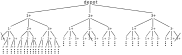
\includegraphics[width=\textwidth]{fig_tree_bus_route}\par
    \label{fig:tree_bus_route}
\end{figure}

Nevertheless, in order to build a function that allows us to have a mapping from each walk to a natural number, thus enumerating all the possible routes of a bus, it is necessary to know, given a depth in the tree, how many leaves are under each vertex of this depth. Once this information is available, the transformation function can be computed in a quite efficient way.

Determining how the tree structure is at each level and altogether how many leaves there are depends exclusively on the load of the bus in a given vertex, it means, it depends on how many requests are being carried and how many still remain to be picked up in a specific moment. The Figure \ref{fig:load_bus_scheme} helps to explain this structure. In this illustration each node represents the load of the bus at the respective level, the further down it gets, the greater its respective depth becomes. The edges under a node tell how many children a vertex with the respective load yields. In this example, at the first level the vehicle is in the depot and therefore empty ($Q=0$), at the second level, i.e. the first passenger pick-up, there are three possibilities that generate a bus load of 1, one possibility for each assigned request. In the next steps, every one of the nodes can either pick up one new passenger, who has not been picked up yet, or drop one of the $q$ passengers, where $q$ is the current vehicle load. Note that, in this example, for reason of simplification, it is assumed that there is \emph{only one passenger per request}, an expansion to \emph{many passengers per request} can be similarly done.

\begin{figure}[H]
	\centering
    \caption{Graph describing the structure of the route tree}
    \includegraphics{fig_load_bus_scheme}\par
    \label{fig:load_bus_scheme}
\end{figure}

From the graph illustrated in the Figure \ref{fig:load_bus_scheme} it is possible to extract two matrices in order to represent the structure, one for the pick-up cases (\emph{edges leaving nodes to the right}) and one for the drop-off cases (\emph{edges leaving nodes to the left}). Respectively, the number on these edges are denoted in the following matrices $Q_{in}$ and $Q_{out}$.

$$
Q_{in} = 
\begin{bmatrix}
3 & 0 & 2 & 0 & 1 & 0\\
0 & 2 & 0 & 1 & 0 & 0\\
0 & 0 & 1 & 0 & 0 & 0\\
0 & 0 & 0 & 0 & 0 & 0
\end{bmatrix}
,
Q_{out} = 
\begin{bmatrix}
0 & 0 & 0 & 0 & 0 & 0\\
0 & 1 & 0 & 1 & 0 & 1\\
0 & 0 & 2 & 0 & 2 & 0\\
0 & 0 & 0 & 3 & 0 & 0
\end{bmatrix}
$$

Each row of the matrix maps a car load, starting from the first row with $Q=0$. Additionally, each column maps a level, starting from the one most at left. So, the element $a^{in}_{ij}$ of the matrix $Q_{in}$ equals the number of children created by a node equivalent to a load $q=i$ with level $j$, that lead to an increase of the load (\emph{pick-up}). Analogously, the element $a^{out}_{ij}$ of the matrix $Q_{out}$ is equal to the number of children, that have a lesser load, yielded by every node with $q=i$ in the $j$-th level (\emph{deliver}). Once again, for the simplification of the explanation, the maximal capacity $Q_k$ of the vehicle is not being considered, but it could be done by simply setting every element in a row $i>Q_k$ to zero.

As already mentioned before, in order to design an algorithm similar to the one in the Section \ref{sec:model-request-bus}, one would need to know at every node of the tree, i.e. every stop of the route, how many leaves there are under this node, i.e. how many combinations still can be done with the rest of the route. For that, a third matrix $Q$ is generated by combining $Q_{in}$ and $Q_{out}$ inside the following algorithm. This new matrix maps in each element $a_{ij}$ the amount of leaf nodes under a vertex with $q=i$ in the $j$-th level.
\begin{algorithm}[H]
\setstretch{1}
\caption{Matrix Generation}
\begin{algorithmic}
\Function{Generate Matrix of Number of Leaf Nodes}{$Q^{in}, Q^{out}$}
\State Let $n$ be the the number of requests and $\odot$ the element-wise multiplication
\State $\displaystyle Q_{2n+1} \gets \begin{bmatrix}1\\ 0 \\ \vdots \\0 \end{bmatrix}$
\For{$i = 2n : 1$}
	\State $\displaystyle Q_{i} \gets Q^{in}_{i} \odot \begin{bmatrix}Q_{i+1,1..n-1} \\ 0\end{bmatrix}
	+ Q^{out}_{i} \odot \begin{bmatrix}0\\ Q_{i+1,2..n}\end{bmatrix}$
\EndFor
\State \Return $Q$
\EndFunction
\end{algorithmic}
\end{algorithm}

The result of applying the function for the matrices $Q_{in}$ and $Q_{out}$ is shown below. The entry $Q_{1,1}$ provides the total number of leaves in the tree, in other words, the number of possible routes for a given vehicle. As a route is codified in the correspondent vector component, the value in $Q_{1,1}$ gives an upper limit for the number interval in which routes for the respective vehicle can be represented. Ultimately, it is also useful for constraint checking and for an easy creation of the initial generation of fireflies.

$$
Q = 
\begin{bmatrix}
90 & 0 & 6 & 0 & 1 & 0 & 1\\
0 & 30 & 0 & 3 & 0 & 1 & 0\\
0 & 0 & 12 & 0 & 2 & 0 & 0\\
0 & 0 & 0 & 6 & 0 & 0 & 0
\end{bmatrix}
$$

With help of these three matrices and given a correspondent vector component value, the path of a bus can be computed by a transformation function. Below is shown a function that takes these arguments and delivers a path performed by a bus, where its elements do not represent the requests themselves, but the vertices of the walk in the tree represented in the Figure \ref{fig:tree_bus_route}, which is relative to each bus. A mapping to the absolute requests can be trivially done once the requests assigned to each bus are known.

To summarize, the procedures explained in this section show that every route of every vehicle can be represented by a unique number. So, the solution vector (i.e. the firefly vector) stores a possible configuration of the vehicle routes. Consequently, the extraction of each vehicle's route from this vector is done by (i) transforming the vector's first component into the mapping of requests to vehicles, as shown in the Section \ref{sec:model-request-bus}; (ii) transforming each one of the following components into a walk in the tree of possible routes, as in the algorithm below; (iii) on the basis of this walk and of the assignment request-vehicle, composing the routes of each vehicle. At last, after this transformation of the vectorial representation of a solution of the DARP into vehicle routes, the only infeasibility that there may exist is concerning time windows and ride time constraints. This will be discussed in subsequent sections.
\begin{algorithm}[H]
\setstretch{1}
\caption{Transformation Vector-Solution}
\begin{algorithmic}
\Function{Transform Component to a Walk in the Tree}{$Q^{in}, Q^{out}, Q, v$}
\State Let $n$ be the the number of requests of the bus
\State $Path \gets [ ]$
\State $row \gets 0$
\State $pointer \gets 0$
\For{$col = 1 : 2n$}
	\State \# Each loop determines the next node of the path
	\State $\mathit{numOfPickupChildren} \gets Q^{in}_{row,col}$
	\State $\mathit{numOfDropoffChildren} \gets Q^{out}_{row,col}$
	\State \# $ChildrenSizes$ has the number of leaf nodes under each children of the current node
	\State $\displaystyle ChildrenSizes = \begin{bmatrix}\underbrace{Q_{row-1,col+1}}_{\mathit{numOfDropoffChildren}-times}
			, \underbrace{Q_{row+1,col+1}}_{\mathit{numOfPickupChildren}-times}\end{bmatrix}$
	\State $\mathit{numOfChildren} = \mathit{numOfPickupChildren} + \mathit{numOfDropoffChildren}$
	\For{$child = 1 : \mathit{numOfChildren}$}
		\State \# Each loop checks whether the $child$ is the next node
		\If{$v - pointer < ChildrenSizes_{child}$}
			\If{$child < \mathit{numOfDropoffChildren}$}
				\State $row \gets row - 1$
			\Else
				\State $row \gets row + 1$
			\EndIf
			\State \# The next node of the path is determined by the variable $child$
			\State \textbf{break}
		\Else
			\State $pointer \gets pointer + ChildrenSizes_{child}$
		\EndIf
	\EndFor
	\State $Path_{col} \gets child$
\EndFor
\State \Return $Path$
\EndFunction
\end{algorithmic}
\end{algorithm}

\subsection{Distance}
For reasons of efficiency of the implementation and in order to keep the numerical error under control, the \textbf{Manhattan distance} was used to approximate the distance between two vectors in the search space. Note that, the Manhattan distance is very convenient for combinatorial applications because, if the vectors are composed by only integer numbers, then its result will be expressed in integer numbers too. The Manhattan distance between two vector $\mathbf{p}$ and $\mathbf{q}$, both with length $n$, is defined as follows.

$$d(\mathbf{p},\mathbf{q}) = \parallel \mathbf{p} - \mathbf{q} \parallel = \sum_{i=1}^{n} \mid \mathbf{p}_{i}-\mathbf{q}_{i} \mid$$

\subsection{Attractiveness}\label{sec:attractiveness}
As proposed by \textcite[p. 173]{yang_firefly_2009}, the attractiveness is calculated with the following quotient, which varies with the squared distance between two vectors.
$$\beta(r) = \frac{\beta_{0}}{1 + \gamma r^2}$$

However, without loss of quality in the method, the attractiveness can vary directly with the distance, as the search space is too large and concerns with numerical errors play an important role. Moreover, due to these concerns, we assume that $\beta_0 = 1$, i.e. the attractiveness at the light source is 100\%, then, we define the inverse function $\beta^{-1}$, which is useful for calculating the displacement of a firefly with a minor error.
$$\beta^{-1}(r) = 1 + \gamma r$$

\subsection{Randomization Term}\label{sec:random_term}
The random term of the metaheuristic movement equation is by default $\alpha \cdot \epsilon$, where $\epsilon \sim N(0,1)$. Though, as stated by \textcite[p. 80]{yang_firefly_2010}, \enquote{it is a good idea to replace $\alpha$ by $\alpha S_k$ where the scaling parameters $S_k (k=1,...,d)$ in the $d$ dimensions should be determined by the actual scales of the problem of interest}. As the size of each dimension of the firefly vector is easily obtainable, these sizes are used in this model as scaling parameters. Moreover, \textcite[p. 37-38]{yang_firefly_2013} present an iterative change of the \emph{alpha} parameter, by varying it according to the optimization evolution $t$. Thus, they introduce a new variable \emph{delta}, so \emph{alpha} is updated by the equation
$$ \alpha_t = \alpha_{t-1} \cdot \delta, (0 < \delta < 1),$$ where $\alpha_0$ is the initial scaling factor. Additionally, the author gives also advice about setting \emph{delta}: \enquote{$\delta$ is essentially a cooling factor. For most applications one can use $\delta = 0.95$ to $0.97$}.

At last, due to the fact that the search space is discrete, it is wanted an integer number for the randomization term. In order to achieve that, rounding is performed, proper concerns about numerical errors were taken in the implementation, so that they are reduced at most.

\subsection{Movement in the Discrete Space}
The movement of a firefly $i$ towards $j$ is determined by the following equation.
$$\mathbf{x^{t+1}_i} = \mathbf{x^{t}_i} + \beta(d(\mathbf{x^{t}_i}, \mathbf{x^{t}_j})) \cdot (\mathbf{x^{t}_j} - \mathbf{x^{t}_i}) + RandomTerm(t)$$

Since the fireflies move in a discrete vector space, the terms of the sum above should also be vectors of integer numbers. The first and the last one are intrinsically in the set of the integers. Despite of that, the second term must be rewritten, so that it delivers an integer number with the lowest possible error. Thus, we use the $\beta^{-1}$ function, defined in the Section \ref{sec:attractiveness}, and turn the multiplication into a division. Lastly, rounding should be performed in the quotient, this is done by applying the floor function. As a result, we obtain the function below.
$$\mathbf{x^{t+1}_i} = \mathbf{x^{t}_i} +  \lfloor \frac{(\mathbf{x^{t}_j} - \mathbf{x^{t}_i})}{\beta^{-1}(d(\mathbf{x^{t}_i}, \mathbf{x^{t}_j}))} \rfloor + RandomTerm(t)$$

It is important however to notice that the movement formula may position a firefly out of the interval where one can find solutions, since every dimension of the search space has a range in which meaningful routes can be generated from the firefly vector. On this issue the so-called \textbf{saturation arithmetic} is applied by \emph{clipping} the result, in other words, if the numerical values resulted from the calculation are outside the domain, i.e. greater than its upper limit or less than zero, then the limit values are taken instead.

Moreover, even if the vector lies inside the mentioned domain, it can still deliver unfeasible solutions due to the time windows and passenger ride time constraints. Likewise, a domain adjustment procedure alters the vector in such a way that it then represents a similar, but feasible, solution. The operation is abstractly exemplified in the Figure \ref{fig:solution_domain}. The graph illustrates one of the domains of the search space, the gray regions characterize ranges of values which hold valid solutions, the point $S_i$ is a component of a vector and $S'_i$ is the new component value after the application of the domain correction procedure.

\begin{figure}[H]
	\centering
    \caption{Illustration of the domain correction procedure}
    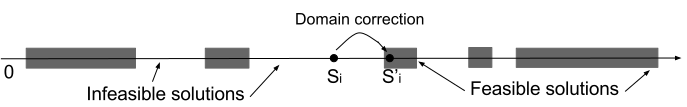
\includegraphics[width=\textwidth]{fig_solution_domain}\par
    \label{fig:solution_domain}
\end{figure}

The \textbf{domain correction procedure} consists in rearranging the routes of every bus, such that the distance between the new vector and the old one is as low as possible. The Figure \ref{fig:tree_bus_route} helps to clarify the situation, it shows how the routes can be represented by a tree, note also that a branch from the root to a leaf describes a possible vehicle route. The objective of the correction function is to find a new branch in the tree, that lies near the unfeasible one. To solve the problem, one can see it as a \textbf{constraint satisfaction problem}, where the set of variables are the request locations, their domains are the possible positions in the route, and the set of constraints are the time window limitations, which tell whether a location must be accessed before or after another one. In this work, the renowned \textbf{Arc Consistency Algorithm \#3} by \textcite{mackworth_consistency_1977} was implemented in order to correct vectors.

To add a final observation, it is to note that, despite of all the effort to correct the firefly vector, the adjustment function may not find a valid route if, for instance, the assignment of requests to vehicles does not make it possible. In this case, the firefly lies out of domain and should have null intensity.

\subsection{Intensity Function}
The intensity function models the brightness of a firefly and should be directly proportional to the utility function of the problem to be maximized. Since the problem's goal is to minimize the operation costs (or the operation time), one could then think of using the \emph{negative cost function} as utility function, what is commonly done when treating optimization problems. However, the firefly algorithm requires a positive function instead, since the intensity is by definition non-negative.

Nevertheless, the cost function has an upper limit, that can be estimated by calculating the worst set of vehicle routes. We propose to sum the distance of the $m$ most distant vertices in the graph G $-$ explained in the Section \ref{sec:integer-programming} $-$ whose vertices are the pick-up and drop-off locations of each passenger and whose edges are the distance between them. Hence, $m$ should be twice the number of requests since every request has two correspondent vertices, one for boarding and one for alighting. Once this value is calculated, the costs of a given solution can be subtracted from it, in order to obtain an utility function. This process is equivalent to translating the negative cost function, i.e. shifting it upwards in the \emph{Cartesian plane}.

So, to start with, assume that the route costs are equal to the route times, then, let $max$ be the mentioned superior cost limit, $n$ the number of requests and $C$ the adjacency matrix, which has the costs between any stop location, note that $C$ is a square matrix with $2n+1$ rows which include the pick-up and delivery locations plus the depot. Finally, let $f$ be a function that, given the solution vector $\mathbf{x}$, returns a binary matrix with the same shape than $C$ and whose elements have the value $1$ if a vehicle travels through the respective edge, and $0$ otherwise. Hence, the intensity function $I$ can be defined in the following formula.
$$I(\mathbf{x}) = \begin{cases} 0, & \text{if }\mathbf{x}\text{ does not meet the constraints}\\
								max - \displaystyle\sum_{i=1}^{2n+1}\sum_{j=1}^{2n+1} f(\mathbf{x})_{i,j} \cdot C_{i,j}, & \text{else}
					\end{cases}$$

\subsection{Initial Solution}
A set of initial solutions is calculated by simply generating for each component of the vector a random natural number in a valid interval. Firstly, the first component is randomized, its range is $[0, k^n)$, where $n$ is the number of requests and $k$ the number of buses. Secondly, the other components are randomized, their domain intervals are determined based on the assignment of requests to buses resulted from the first component randomization. In this way, the first generation of fireflies can be efficiently created. Note that, there is no guarantee that these are feasible solutions, yet it does not pose an issue, since these vectors will be corrected throughout the algorithm's iterations.

\subsection{Parameters}
The choice of the parameters is basically based on the work of \textcite[p. 37-38]{yang_firefly_2013}. For that, the scale $L$ of the problem is taken into consideration, it represents namely the size of the search space and is calculated by multiplying the sizes of the intervals of each dimension, in which the intensity function is defined. The parameter \emph{gamma} is then set $\gamma = 1/\sqrt{L}$. In order to have a broad exploration of the space, we set $\alpha_0 = 0.1$, the parameter will be then reduced along the optimization process. Lastly, we set $\beta_0 = 1$, $\delta = 0.95$ and the number of fireflies to 40.

Regarding the stop criteria, the algorithm stops if there is no improvement of the best solution after 200 iterations or the algorithm has executed 1000 iterations, whatever comes first.

\subsection{Two-Phase Optimization}
It is to note that, in a regular problem instance, the assignment of requests to vehicles has a great weight in the cost function. Empirical observations suggest that this assignment is roughly the most determinant factor in the calculation of the costs. For instance, grouping requests that are geographically near tends to show better results regardless of the route configurations. Yet the route of each vehicle plays an important role in finding an optimal result.

Moreover, as the contribution to the cost function by the vector components that describe each bus' route is strongly dependent on which requests each bus is allocated to, it makes no sense trying to optimize vehicle routes in a stage where the assignment request-bus shows a large deviation from iteration to iteration.

On the basis of these observations, an optimization process with two phases is performed. In the model presented here, there is a first stage, where only the first vector component is optimized by moving the fireflies only in this dimension of the search space. In a second stage, the other components are optimized by anchoring the first component and allowing the movement of the fireflies in these other dimensions.

The Figure \ref{fig:alpha_evolution} displays the evolution of the alpha parameter $-$ described in the Section \ref{sec:random_term} $-$ in the two-phase optimization process. The X-axis shows the iteration sequence, while the Y-axis shows the value of alpha in the respective iteration, which is scaled, in the first phase, according to the first dimension's range, and, in the second phase, according to the range of the other dimensions.

\begin{figure}[H]
	\centering
    \caption{Evolution of the alpha parameter}
    \includegraphics[width=\textwidth]{fig_alpha_evolution}\par
    \label{fig:alpha_evolution}
\end{figure}

\subsection{Implementation}
One of the main difficulties in implementing the algorithm is the magnitude that the numbers might assume. To workaround the problem the programming language \emph{Python} was chosen due to its native implementation of integers with unlimited size. Besides, the proposed model has a considerable quantity of matrix operations, therefore, the libraries \emph{NumPy} and \emph{Scipy} were used for that purpose. For drawing the graphs it was adopted the library \emph{Matplotlib}, which has an easy-to-use interface for the programmer.

A special concern with the numerical operations and the data types had to be taken to ensure no integer overflows and a controlled numerical error at the lowest level.

To obtain a better performance and to have the most recent features available, the implementation was developed and executed on the newest possible tool versions, namely, the versions 3.4 of \emph{Python}, 1.10 of \emph{NumPy}, 0.16 of \emph{SciPy} and 1.3 of \emph{Matplotlib}.

The Figure \ref{fig:output} shows an example of some of the outputs given by the implemented program, it displays the routes of two vehicles in a xy-plane. In each graph, the black dot represents the depot and the red dots represent the drop-off stops, while the blue and the green dots are pick-up stops.
\begin{figure}[H]
	\centering
    \caption{Example of output by the program}
    \begin{subfigure}[b]{0.49\textwidth}
	    \includegraphics[width=\textwidth]{fig_output1}
    \end{subfigure}
    \begin{subfigure}[b]{0.49\textwidth}
	    \includegraphics[width=\textwidth]{fig_output2}
    \end{subfigure}\par
    \label{fig:output}
\end{figure}

The Figure \ref{fig:best-solution-evolution} illustrates how the current best solution evolves along the algorithm's execution with a test input. Observe that the Y-axis represents the utility function instead of the costs.
\begin{figure}[H]
	\centering
    \caption{Evolution of the current best solution along the iterations}
    \includegraphics[width=0.9\textwidth]{fig_best_sol_evolution}\par
    \label{fig:best-solution-evolution}
\end{figure}

%============================================================
% Chapter 5. Evaluation
%============================================================
\chapter{Evaluation}\label{sec:evaluation}
The objective of this chapter is to evaluate the proposed implementation of the firefly metaheuristic by running it with several problem instances as input. The characteristics that are taken into consideration are the \textbf{result quality}, that is to say, how far the calculated cost for the best solution found is from the instance's optimal solution, the \textbf{algorithm progress}, which tells how better the best solution found is in comparison to the initial solution, and, at last, the \textbf{running time}.

Two distinct types of experiments are carried out. In the first place, the firefly approach is compared against the generic solver by executing both programs with the same inputs. With it, it is expected to asses to what extent the metaheuristic implementation outperforms the generic solver. In the second place, the near-optimal approach is tested with instances that are recurrently used in the literature. Similarly, the deviation of the solution to the optimum and the program processing time are evaluated and compared to state-of-the-art methods.

In the total, the experiments include 24 instances which are solved in a computational environment with a 64bits \emph{Intel Xeon} CPU at 2.3 GHz, 15 GB of main memory and a \emph{Python} interpreter version 3.4 on a \emph{Linux} operating system.

\section{Results and Discussion}
First of all, we wanted to evaluate the exact approach through the integer programming solver GLPK and how it performs in comparison to the near-optimal implementation. The instances were then executed with a memory limit of 7 GB. But, as one could have expected, the generic solver was not able to solve even the smallest instance, \emph{a2-16}, neither could a feasible, non-optimal solution be found. Therefore, in order to present results of comparison, the instance \emph{a2-16} was reduced in several smaller ones, with number of requests between 3 and 8.

The results are shown in the Figure \ref{tab:evaluation-1}, which summarizes the values that we are interested in. In the columns \emph{Req}, \emph{Bus} and \emph{Cap} are listed the features \emph{number of requests}, \emph{number of buses} and \emph{vehicle capacity}, respectively, for each instance. The columns \emph{Opt.} and \emph{CPU-GLPK} display the costs of the optimal solution found by the generic solver and the CPU time in minutes, respectively. The columns \emph{Firefly Sol.} and \emph{\% Opt.} show the solution found by the metaheuristic approach and its deviation to the optimum, this is calculated by simply dividing the value in \emph{Opt.} by the one in \emph{Firefly Sol}. Finally, the time in minutes of the solution through the firefly algorithm can be seen in the last column.
\begin{table}[H]
\centering
\caption{Results of the first evaluation}
\setstretch{1}
\begin{tabular}{l | r | r | r | r | r | r | r | r}
\hline
Inst. & Req & Bus & Cap & Opt. & CPU-GLPK & Firefly Sol. & \% Opt. & CPU-Firefly\\
\hline
Test-1 & 	3 & 	2 & 	3 & 	58.05 & 	0.1 & 	69.75 & 	83.2\% & 	7.4 \\
Test-2 & 	4 & 	2 & 	3 & 	68.10 & 	0.9 & 	98.51 & 	69.1\% & 	11.7 \\
Test-3 & 	5 & 	2 & 	3 & 	76.27 & 	2.0 & 	134.29 & 	56.8\% & 	2.5 \\
Test-4 & 	6 & 	2 & 	3 & 	96.54 & 	45.0 & 	149.32 & 	64.6\% & 	3.3 \\
Test-5 & 	8 & 	2 & 	3 & 	- & 	- & 	158.67 & 	- & 	5.7 \\
\hline
\end{tabular}
\label{tab:evaluation-1}
\end{table}

Note that, because it had reached the execution limit, the exact approach could not solve the instance \emph{Test-5} of the experiment. This fact together with the growth of CPU time required for the GLPK to solve instances as they become bigger suggest an exponential increase in use of resources (e.g. processing time and memory) that the exact solver consumes. All in all, it confirms what one would generally expect in the case that the growth of the input entails the increase in the number of dimensions of the solution space: the so-called \emph{Bellman's curse of dimensionality}\footnote{See Bellman, Richard E. 2003. Dynamic Programming.  Courier Corporation.}

In light of the results, one can conclude that, on the one hand, GLPK is very effective for small instances, but on the other hand, due to its high complexity of both time and space, it is not capable of being applied for larger inputs, as in real-world applications. As opposed to that, the solution with the metaheuristic may be not so effective in delivering the optimal result. However, due to its robustness, its efficiency when solving larger instances lies way above the exact approach. This can be clearly seen in the column \emph{CPU-Firefly}, whereby the algorithm's computational time presents a relatively small variation and appears to have a steady growth as the inputs become larger. This observation is supported by the subsequent experiments.

The second conducted evaluation analyzed the following three aspects of the problem solver that implemented the firefly algorithm: (i) how close to the optimum the metaheuristic approach can reach, i.e. the solution quality; (ii) how the solutions are improved from the initial feasible solution until the final one, this indicates to what extent the optimization method in fact helps minimizing the cost function; (iii) how, in a temporal perspective, the application behaves regarding the increase in the input size.

From the total of 24 instances 15 could be solved, the results regarding the quality and progress are presented in the Table \ref{tab:evaluation-2.1}. The two first columns describe the characteristics of the data inputs, respectively name and optimal solution. The columns \emph{Final Sol.} and \emph{Optimality} show the best solution found and its proportion with respect to the instance optimum. The two last columns refer to the progress of the solutions, in \emph{Initial Sol.} is the first yielded feasible solution and in \emph{Dev. to Initial Sol.} is the deviation of the final result to the initial one, it is calculated by dividing the difference between these two values by the initial solution, in formula: $\textit{ Dev. to Initial Sol.} = (\textit{Initial Sol.} - \textit{Final Sol.}) / \textit{Initial Sol.}$.
\begin{table}[H]
\centering
\caption{Results of the second evaluation $-$ Quality and progress}
\setstretch{1}
\begin{tabular}{l | r | r | r | r | r}
\hline
Instance & Optimum & Final Sol. & Optimality & Initial Sol. & Dev. to Initial Sol.\\
\hline
a2-16 & 	294.25 & 	312.96 & 	94.02\% & 	335.85 & 	6.81\% \\
a2-20 & 	344.83 & 	373.89 & 	92.23\% & 	427.48 & 	12.54\% \\
a2-24 & 	431.12 & 	442.85 & 	97.35\% & 	496.92 & 	10.88\% \\
a3-18 & 	300.48 & 	347.10 & 	86.57\% & 	374.20 & 	7.24\% \\
a3-24 & 	344.83 & 	409.73 & 	84.16\% & 	456.86 & 	10.32\% \\
a3-30 & 	494.85 & 	614.13 & 	80.58\% & 	615.99 & 	0.30\% \\
a3-36 & 	583.19 & 	- & 	- & 	- & 	- \\
a4-16 & 	282.68 & 	310.84 & 	90.94\% & 	354.54 & 	12.33\% \\
a4-24 & 	375.02 & 	481.16 & 	77.94\% & 	567.63 & 	15.23\% \\
a4-32 & 	485.50 & 	639.73 & 	75.89\% & 	665.27 & 	3.84\% \\
a4-40 & 	557.69 & 	780.13 & 	71.49\% & 	841.92 & 	7.34\% \\
a4-48 & 	668.82 & 	956.90 & 	69.89\% & 	1032.38 & 	7.31\% \\
a5-40 & 	498.41 & 	779.32 & 	63.95\% & 	818.14 & 	4.74\% \\
a5-50 & 	686.62 & 	926.23 & 	74.13\% & 	1018.84 & 	9.09\% \\
a5-60 & 	808.42 & 	1195.94 & 	67.60\% & 	1257.38 & 	4.89\% \\
a6-48 & 	604.12 & 	993.08 & 	60.83\% & 	1025.55 & 	3.17\% \\
\hline
\end{tabular}
\label{tab:evaluation-2.1}
\end{table}

Note that it was not possible to find a solution for the instance \emph{a3-36}. That is mainly due to the fact that it has a high rate of request per vehicle. As one can see in the Table \ref{tab:instances-attributes}, it implies that, with a higher number of requests in a bus route, it becomes very often impossible to arrange the locations in an order that fulfills the problem's constraints. On this issue, one should take into consideration, that there are two distinct tasks that are affected by the density of request per bus, firstly, the assignment of requests to buses, secondly, the arrangement of each bus' route. Then, as the former is performed merely randomly, the algorithm of domain correction, which is applied solely to the routes, can be quite ineffective since the desired effect depends broadly on the assignment of requests to the route.

When considering the optimality of the results, one can ascertain that the implementation delivers very good solutions to the smaller instances, for example, from the instance \emph{a2-16} until the instance \emph{a4-16} the mean value for the optimality is approximately 90\%. The other outcomes, whose optimalities lie below the percentage of 80\%, have a performance that should already be expected, since, in these cases, the search space becomes very large due to its high dimensionality. Besides, the sparseness of the regions of feasible solutions increase in such a way, that the interaction between the fireflies becomes less and less frequent, thus, almost annulling the optimization process.

Moreover, the balance between \emph{exploration} and \emph{exploitation} plays an important role. A policy of exploration tends to lead the optimization process away from local optima, avoiding low quality solutions, at the expense of increasing the processing time. By contrast, a policy of exploitation tends to a local search, delivering impaired solutions, but in a short period of time. To sum up, whether the solution of an instance has a better or worse quality depends also on this balance, the optimality can in some cases eventually be improved, though the price that one have to pay might be unwanted.

At last, the progress from a feasible initial solution to the best solution has presented a variation at the experiments, namely from 0.3\% to over 15\%. That is mostly because of the domain correction procedure performed with the randomly distributed vectors of the initial solutions. Since the set of initial solutions happens to be high probably invalid, they pass through the domain adjustment algorithm, whose heuristic for forming the feasible route may eventually be good enough to place the vector very close to the optimum, causing a low deviation of the final solution.

The Table \ref{tab:evaluation-2.2} makes a comparison between the computing times taken by the experiments and the computing times of two solvers from the literature. In the columns \emph{CPU$^1$} and \emph{CPU$^2$} are the processing times of the solutions by \textcite{parragh_introducing_2011} and by \textcite{parragh_hybrid_2013}, respectively. Some CPU times were not included in the respective papers, these are then marked with a dash (-) in the respective cell of the table. Finally, the column \emph{CPU-Firefly} illustrates the results of the experiments realized by this work. In bold are highlighted the ones which executed faster than the solution of \textcite{parragh_introducing_2011}.
\begin{table}[H]
\centering
\caption{Results of the second evaluation $-$ Running time}
\setstretch{1}
\begin{tabular}{l | r | r | r}
\hline
Instance & CPU$^1$ & CPU$^2$ & CPU-Firefly\\
\hline
a2-16 & 	68.2 	& 	0.12 & 	\textbf{63.3} \\
a2-20 & 	133.8 	& 	0.28 & 	160.5 \\
a2-24 & 	187.8 	& 	0.35 & 	419.3 \\
a3-18 & 	45.4 	& 	- & 	\textbf{29.5} \\
a3-24 & 	86.8 	& 	0.29 & 	\textbf{77.4} \\
a3-30 & 	105.6 	& 	0.50 & 	151.2 \\
a3-36 & 	162.6 	& 	0.83 & 	370.6 \\
a4-16 & 	26.0 	& 	- & 	\textbf{14.5} \\
a4-24 & 	50.8 	& 	- & 	\textbf{37.0} \\
a4-32 & 	86.0 		& 	0.55 & 	129.4 \\
a4-40 & 	130.6 	& 	0.78 & 	233.5 \\
a4-48 & 	253.8 	& 	1.62 & 	\textbf{222.3} \\
a5-40 & 	- & 	0.85 & 	156.8 \\
a5-50 & 	- & 	1.60 & 	366.1 \\
a5-60 & 	- & 	2.51 & 	323.1 \\
a6-48 & 	- & 	1.14 & 	146.7 \\
a6-60 & 	- & 	2.29 & 	279.3 \\
a6-72 & 	- & 	4.43 & 	648.7 \\
a7-56 & 	- & 	1.67 & 	186.2 \\
a7-70 & 	- & 	2.88 & 	348.5 \\
a7-84 & 	- & 	7.04 & 	553.5 \\
a8-64 & 	- & 	2.14 & 	101.8 \\
a8-80 & 	- & 	5.73 & 	203.7 \\
a8-96 & 	- & 	9.92 & 	477.4 \\
\hline
\end{tabular}
\label{tab:evaluation-2.2}
\end{table}

As one can see, concerning processing time, the firefly implementation shows results equivalent to the approach of  \textcite{parragh_introducing_2011}. In comparison, our implementation outperforms the latter in approximately half of the cases. Unfortunately, the desired efficiency of the state-of-the-art method could not be achieved. A possible reason for that is the sparseness of the feasible solution in the search space, which is so extreme that almost every firefly movement operation results in infeasibility, because of that, the domain correction algorithm ends up by taking a large proportion of execution time. A second cause for the undesired efficiency is the amount  of numerical operations with very large integers, which are performed due to the designed representation of the solution and which cannot be natively performed by the computer.

In general, the improvement of the code of the implementation could ultimately improve the numerical results presented above. However, it would not change the overall perspective of the approach in comparison with the other ones from the literature.

%============================================================
% Chapter 6. Conclusion
%============================================================
\chapter{Conclusion}
First of all in this research, the state-of-the-art and the approaches proposed in the literature of the Dial-a-ride problem (DARP) were studied. The so-called two-index mathematical formulation was chosen to serve as the definition of the optimization problem, which was afterwards transcribed into a programming language, namely \emph{AMPL}, interpreted and executed by the generic solver \emph{GLPK}. Secondly, the firefly algorithm (FA) was implemented as a metaheuristic approach to solve the DARP with the assumption that it would outperform the generic solver in cases of larger inputs. Finally, both methods to solve the problem were evaluated through experiments, which were carried out with the instances that are utilized in the literature with the purpose of assessing the outcomes.

We started with the premise that the GLPK would not be capable of being applied in the practice due to the combinatorial growth of the solution space that larger instances of the problem can generate. As expected, the evaluation results corroborates this statement, since the generic solver could merely deliver solutions for very small instances, smaller than the simplest one of our dataset.

Therefore, we assumed that a metaheuristic implementation was necessary in order to be able to overcome the challenges imposed by the complexity of the DARP. The recently-conceived firefly algorithm seemed to be suitable for this purpose, mainly because this technique creates several initial solutions, which are spread over the multidimensional space, and which interact with each other towards the convergence to an optimal result. The program showed satisfactory answers by solving larger instances than those which the GLPK was capable of, and in some cases reaching optimality of over 90\%.

In addition, in order to asses our method with the current scientific perspective, we put its execution time in comparison to state-of-the-art techniques. As a result, it turned out to deliver some results as fast as one of the considered algorithms, what evidences its possible applicability.

Concerning the context of the DARP, it has been mostly applied to the transportation of disabled people by small vehicles, who can use this flexible service instead of a taxi, what in turn implies significantly higher costs to those people. Working on the problem contributes towards the improvement of the current public transportation in both small and large towns. Besides, approaching the DARP as an optimization problem allows the organizations, that act in the branch, to guarantee a good cost-benefit relationship in the operation of such a service.

Furthermore, none of the works found in the literature tried to solve the problem with swarm intelligence. In this sense, this work proposed a novel approach for addressing the DARP, using the firefly metaheuristic, which had already succeeded in solving the traveling salesman problem \parencite{jati_evolutionary_2011}.

Another contribution to the field is the vectorial representation of the solution, whose components are directly related to the problem features, such as the routes of each vehicle or the assignment of requests to vehicles. On the one hand, this makes possible to easily operate with the vectors, on the other hand, this implies in extra computational costs by having to transform the vector for every evaluation of the objective function.

Besides, in order to obtain feasible solutions, the problem of correcting the firefly vectors had to be tackled. The idea of seeing it as a constraint satisfaction problem and solving it with the AC-3 algorithm was a new way of treating the issues regarding the many constraints, which arise when designing routes for the vehicles in the DARP.

In summary, the model presents however some bottlenecks, the main one is the large amount of infeasible regions in the search space, what causes the implemented program to spend a lot of time correcting the solutions that fall into such regions. Besides, because of this, it is extremely hard finding feasible solutions for large instances. The workaround for this issue would be suitable for further research. A simple suggestion would be applying a correction not only to the dimensions related to the vehicle routes, as it was done in this work, but also for the request-vehicle assignment dimension. However, a more effective approach would actually reinvent the model of the solution space, in such a way that invalid regions would not exist at all, in this way, both the processing time and the optimality of the results could be drastically improved.

Furthermore, the evaluation of the objective function for a given solution represents also a high computational effort, thus, a second point for future research would be developing an efficient way to realize the vector transformations required to calculate the route costs, or rather creating a totally new way to evaluate the objective function. Finally, the method could significantly benefit from a parallel implementation of the FA or from a multiagent-oriented approach.

To sum up, we presented a model together with a prototype to solve the Dial-a-ride problem, which showed solutions comparable to state-of-the-art methods. After all, the knowledge generated from this research indicates to be consistent, indeed, with some betterments it would stay not very far from practical applications.
%============================================================
% Chapter 6. Conclusion
%============================================================
\nocite{*}
%\bibliographystyle{abntex2-alf}
\printbibliography

\end{document}
